% ============================================
% РАЗДЕЛ 2. ПРОЕКТИРОВАНИЕ КАСКАДНОЙ АРХИТЕКТУРЫ
% ============================================

\section{Проектирование каскадной архитектуры системы распознавания голосовых команд}

В разделе~1 на основании анализа предметной области сформулирована
гипотеза о возможности достижения энергоэффективности KWS-системы на
микроконтроллере общего назначения за счёт совместного применения
каскадной архитектуры детекции и квантизации нейросетевой модели, а
также определены требования, которым должно удовлетворять проектируемое
решение. Настоящий раздел посвящён формализации методологии каскадного
управления режимами энергопотребления, выводу проектных критериев
выбора параметров каскада, обоснованию архитектуры и гиперпараметров
нейросетевого классификатора, а также описанию применяемых методов
квантизации.

\subsection{Принцип каскадной детекции и формализация энергобюджета}

Идея каскадной детекции состоит в разделении задачи непрерывного
мониторинга звукового потока на последовательность ступеней с
возрастающей вычислительной сложностью и, как следствие, возрастающим
мгновенным энергопотреблением. Каждая ступень выполняет функцию
фильтра-предусловия: она активирует следующую ступень только при
срабатывании по своему, более простому критерию. В периоды абсолютной
тишины работает только первая, наиболее дешёвая ступень; вычислительно
затратные операции~--- извлечение признаков и нейросетевой инференс~---
выполняются лишь по событию, потенциально содержащему голосовую команду.

Преимущество каскадной архитектуры перед режимом непрерывного инференса
обусловлено асимметрией активности ступеней во времени. Пусть система
состоит из $K$ последовательных ступеней с мгновенным потреблением
мощности $P_1, P_2, \ldots, P_K$ соответственно ($P_1 \ll P_2 < \ldots
	< P_K$). Обозначим $\alpha_k$ долю времени, в течение которой ступень
$k$ находится в активном состоянии. Первая ступень активна всегда:
$\alpha_1 = 1$. Каждая последующая ступень активируется только при
срабатывании предыдущей, поэтому $\alpha_{k+1} = \alpha_k \cdot
	p_{k}^{\mathrm{trig}}$, где $p_{k}^{\mathrm{trig}}$~--- вероятность
активации ступени $k+1$ по результату работы ступени $k$ за единицу
времени. Средняя потребляемая мощность системы выражается в виде

\begin{equation}
	\bar{P} = \sum_{k=1}^{K} \alpha_k \cdot P_k,
	\label{eq:cascade_power}
\end{equation}

где $\bar{P}$~--- средняя мощность системы за длительный промежуток
наблюдения; $\alpha_k$~--- доля времени активности $k$-й ступени;
$P_k$~--- мгновенная мощность $k$-й ступени в активном состоянии.

В вырожденном случае непрерывного инференса каскад состоит из одной
ступени, постоянно активной, и средняя мощность равна $P_K$. В
каскадной архитектуре при правильно выбранных порогах срабатывания
$\alpha_k$ убывают с ростом $k$ на порядки: для типичного бытового
сценария ($K = 3$, редкие голосовые события) характерны значения
$\alpha_2 \sim 10^{-2}$ и $\alpha_3 \sim 10^{-3}$. Подставляя эти
значения в~\eqref{eq:cascade_power}, нетрудно убедиться, что доминирующий
вклад в среднюю мощность даёт первая ступень~--- даже если её мгновенное
потребление мало по сравнению со всеми остальными.

Из формулы~\eqref{eq:cascade_power} непосредственно вытекают \textit{два
	проектных критерия} каскадной архитектуры, которыми руководствуется
настоящая работа.

\textit{Критерий разделения по сложности.} Чтобы каскадная архитектура
обеспечивала выигрыш относительно непрерывного инференса, мгновенное
потребление каждой ступени должно быть кратно ниже потребления
последующей: $P_k \ll P_{k+1}$. В противном случае энергия, расходуемая
на постоянно активную дешёвую ступень, превзойдёт экономию от редкой
активации дорогой. Применительно к настоящей работе: первая ступень
(аналоговый детектор) должна потреблять не более единиц миллиампер при
напряжении питания целевой платформы, тогда как ступень нейросетевого
инференса допускает потребление в десятки миллиампер при условии её
эпизодической активации.

\textit{Критерий частотного разделения.} Чтобы каскад имел смысл, частота
активации каждой последующей ступени должна быть существенно ниже
частоты активации предыдущей: $\alpha_{k+1} \ll \alpha_k$. Это
обеспечивается тем, что критерий срабатывания ступени $k$ намеренно
выбирается грубее критерия ступени $k+1$: ступень $k$ может допускать
ложные срабатывания, но не должна давать ложных отказов. Все ложные
срабатывания ступени $k$ будут отфильтрованы на ступени $k+1$, тогда как
ложный отказ означает потерю команды и неприемлем.

В настоящей работе принята архитектура с $K = 3$ ступенями. Выбор
именно трёх ступеней обусловлен сочетанием технических ограничений
платформы ESP32-S3 и характера задачи: одноступенчатая архитектура
сводится к непрерывному инференсу; двухступенчатая (аналоговый VAD~---
нейросетевой инференс) объединяет в одной ступени захват аудио,
предобработку и инференс, что не позволяет разделить их вклад в
энергобюджет; трёхступенчатая архитектура разделяет потенциально
наиболее затратный этап (захват и MFCC-предобработка) и собственно
нейросетевой инференс, что соответствует наблюдению Cerutti и
др.~\cite{src:7} о доминирующем вкладе предобработки в общий энергобюджет
KWS-конвейера.

\subsection{Архитектура каскада из трёх ступеней}

Концептуальная схема предложенной архитектуры приведена на
рис.~\ref{fig:cascade_concept}. Каскад состоит из трёх последовательных
ступеней с возрастающей вычислительной сложностью и согласованным
управлением режимами питания микроконтроллера.

\begin{figure}[H]
	\centering
	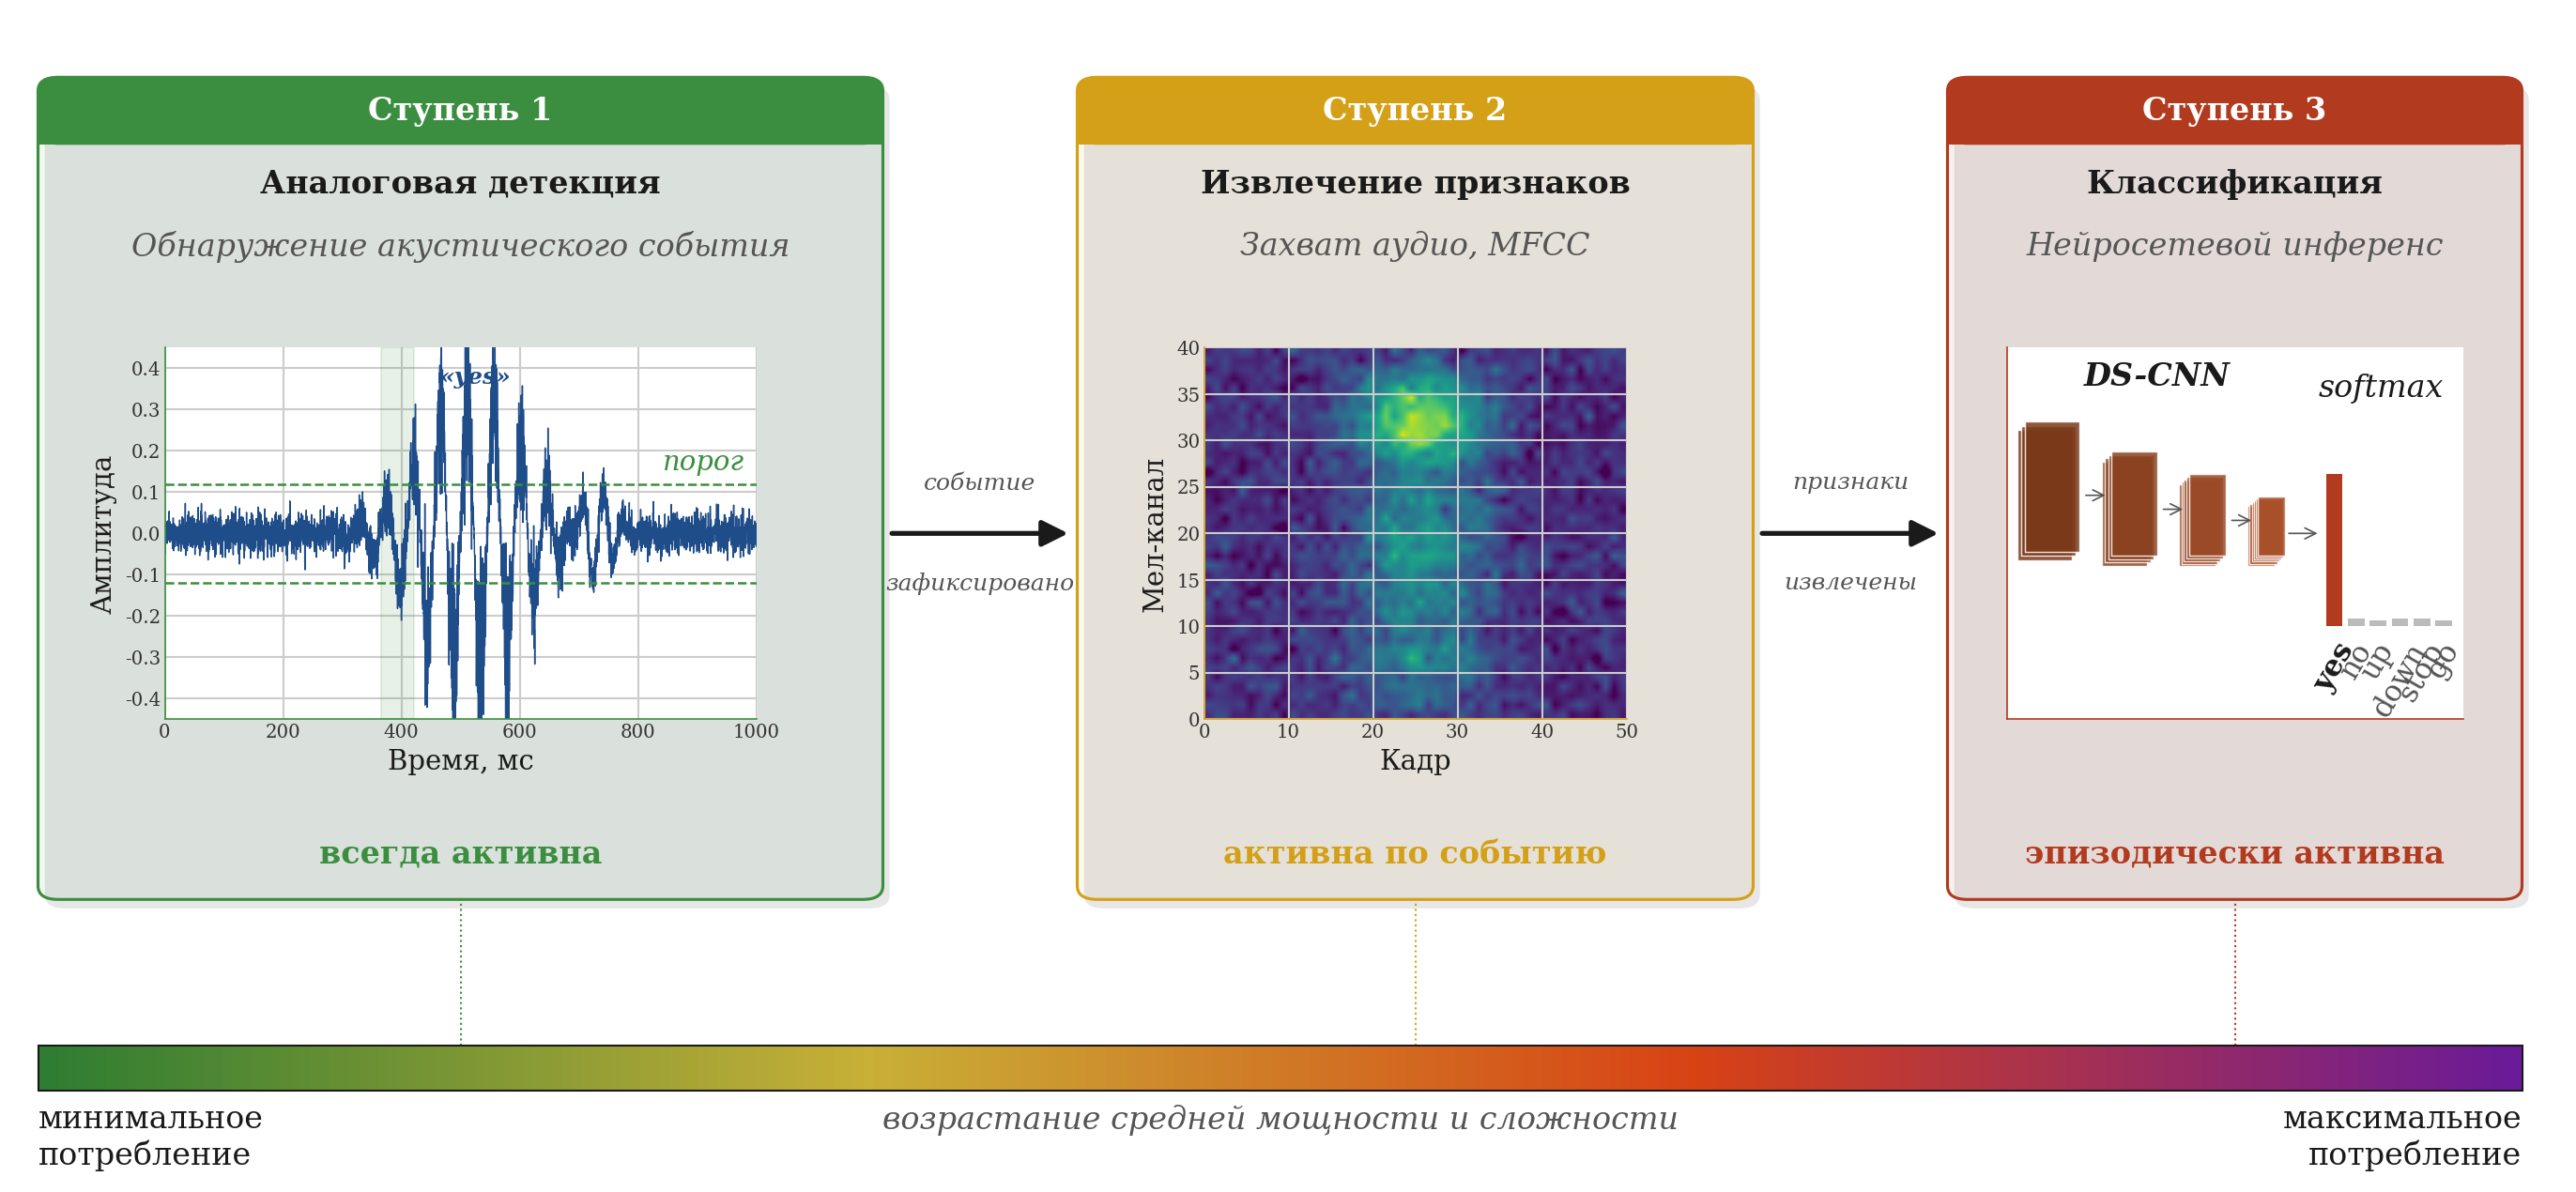
\includegraphics[width=1\textwidth]{assets/images/vad_concept.png}
	\caption{Концептуальная схема каскадного пробуждения: три ступени возрастающей вычислительной сложности с переключением режимов питания микроконтроллера}
	\label{fig:cascade_concept}
\end{figure}

\textit{Ступень~1~--- аналоговая детекция акустического события}~---
выполняет непрерывную пороговую обработку амплитуды сигнала с
аналогового микрофона и принимает решение о наличии звукового
события произвольной природы (речь, шум, удар). Реализована на
маломощном компараторе, потребление измеряется единицами сотен
микроампер, активна постоянно. Положительное решение ступени
формирует аппаратное прерывание, пробуждающее микроконтроллер
из режима глубокого сна.

\textit{Ступень~2~--- захват аудио и извлечение признаков}~---
выполняет запись окна аудио заданной длительности с цифрового
микрофона и расчёт MFCC-признаков на ЦПУ микроконтроллера в
активном режиме. Потребление возрастает до десятков миллиампер,
ступень активна по событию ступени~1 (доли процента общего
времени работы).

\textit{Ступень~3~--- нейросетевая классификация}~--- выполняет
инференс квантизованной DS-CNN с аппаратным SIMD-ускорением и
возвращает индекс распознанного класса. Потребление сопоставимо
со ступенью~2 (десятки миллиампер), ступень активна эпизодически
по результату ступени~2.

Цветовая шкала на рисунке отражает рост средней мощности и
вычислительной сложности от первой ступени к третьей. Указанное
кратное разделение ступеней по мгновенному потреблению и по доле
активности~--- два необходимых условия выигрыша каскадной
архитектуры, формально получаемые из аналитической модели средней
мощности (см. подраздел~\ref{subsec:power_model}).

\subsection{Критерий выбора порога ступени-предусловия}

Каждая ступень-предусловие характеризуется порогом срабатывания,
определяющим компромисс между двумя видами ошибок: ложными
срабатываниями (срабатывание в отсутствие команды, приводящее к
избыточному пробуждению последующих ступеней) и ложными отказами
(несрабатывание при наличии команды, приводящее к её потере).

Для ступени~1 порог компаратора $V_{\mathrm{th}}^{(1)}$ задаётся
аппаратно с помощью подстроечного резистора. Выбор порога производится
экспериментально из условия гарантированного срабатывания при
произнесении команды на типичном для целевого сценария расстоянии от
микрофона и одновременно минимизации срабатываний на фоновый
акустический шум помещения. Поскольку аналоговый компаратор не различает
тип звукового события, ложные срабатывания на бытовые шумы (хлопки
дверей, шаги, посторонняя речь) принципиально неустранимы на данной
ступени; их фильтрация возложена на ступень~3.

Для ступени~3 порог уверенности $\tau_{\mathrm{conf}}^{(3)}$
устанавливается на этапе развёртывания модели в виде минимального
значения логита (или, эквивалентно, вероятности после
softmax-нормализации) победившего класса. Поднятие порога снижает долю
ложных срабатываний ($\mathrm{FAR}$, false acceptance rate), но
увеличивает долю ложных отказов ($\mathrm{FRR}$, false rejection rate);
опускание порога даёт обратный эффект. В контексте каскадной архитектуры
с батарейным питанием приоритет отдан минимизации ложных срабатываний:
каждое ложное срабатывание ступени~3 приводит к ошибочной активации
управляющего действия (например, включение исполнительного устройства),
тогда как ложный отказ требует от пользователя лишь повторить команду.
Тем самым проектное правило формулируется следующим образом: порог
$\tau_{\mathrm{conf}}^{(3)}$ выбирается из условия $\mathrm{FAR} \to
	\min$ при ограничении $\mathrm{FRR}$ сверху заданным значением, не
превышающим ожидаемой комфортной частоты повторов пользователем.

\subsection{Архитектура нейросетевой модели и обоснование гиперпараметров}

В разделе~1 в качестве архитектуры классификатора обоснована
DS-CNN~\cite{src:1}~--- свёрточная сеть с разделимыми по глубине
свёртками. В настоящем подразделе обосновывается конкретный выбор
гиперпараметров модели в рамках предложенного авторами Hello
Edge~\cite{src:1} семейства конфигураций.

В исходной работе~\cite{src:1} предложены три конфигурации,
привязанные к ресурсным ограничениям целевых платформ:

\begin{itemize}
	\item DS-CNN-S (Small): порядка 80~КБ памяти и 6~миллионов операций
	      умножения с накоплением на инференс;
	\item DS-CNN-M (Medium): порядка 200~КБ памяти и 20~миллионов
	      операций умножения с накоплением на инференс;
	\item DS-CNN-L (Large): порядка 500~КБ памяти и 80~миллионов
	      операций умножения с накоплением на инференс.
\end{itemize}

Для настоящей работы выбрана конфигурация DS-CNN в варианте Medium.
Конфигурация Small демонстрирует точность ниже 94\% на наборе Google
Speech Commands~\cite{src:1}, что недостаточно для практического
применения с приоритетом минимизации ложных срабатываний; конфигурация
Large обеспечивает прирост точности менее одного процентного пункта
относительно Medium при четырёхкратном увеличении вычислительной
сложности, что в каскадной архитектуре прямо транслируется в увеличение
длительности и энергопотребления ступени~3. Конфигурация Medium
обеспечивает баланс между точностью и вычислительной стоимостью.

Структурная схема выбранной модели приведена на
рис.~\ref{fig:dscnn_arch}. Входным тензором является матрица
MFCC-признаков размером $49 \times 10 \times 1$. Сеть включает
первичный свёрточный слой (Conv2D, ядро $10 \times 4$, 172 фильтра,
шаг $(2, 2)$), выполняющий начальное извлечение крупномасштабных
спектрально-временных паттернов; шесть блоков разделимой свёртки
(DS-Conv), каждый из которых состоит из depthwise-свёртки с ядром
$3 \times 3$, нормализации (batch normalization), активации ReLU,
pointwise-свёртки с ядром $1 \times 1$, повторной нормализации и
ReLU; глобального усреднения по пространственным размерностям
(Global Average Pooling), обеспечивающего инвариантность к малым
временным сдвигам произнесения команды; полносвязного
классификационного слоя $172 \times 12$. Общее число параметров
модели составляет порядка 300~тысяч, что в формате INT8 после
квантизации соответствует размеру TFLite-файла порядка 260~КБ.

\begin{figure}[h!]
	\centering
	% TODO: НЕ ГОТОВО! сделать нормальную структурную схему DS-CNN-M.
	% Блоки слева направо или сверху вниз:
	% [Input 49×10×1] → [Conv2D 10×4, 172 фильтра, stride 2×2] → [BN+ReLU]
	% → [DSConv ×6] (раскрыть один блок отдельно: DW 3×3 → BN+ReLU → PW 1×1 → BN+ReLU)
	% → [GAP] → [Dense 12] → [Softmax]
	% Сделать в draw.io.
	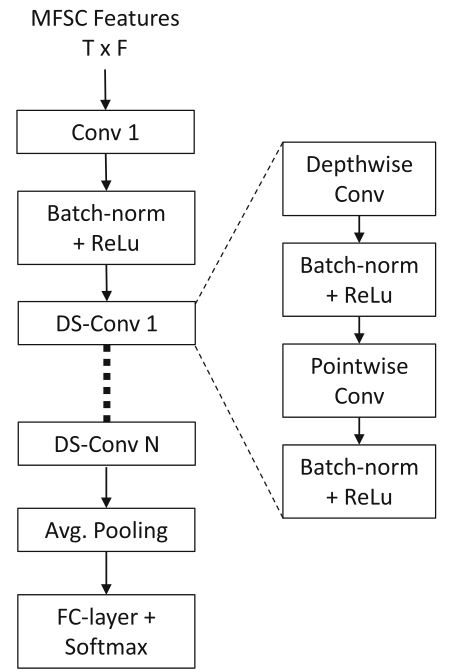
\includegraphics[width=0.6\textwidth]{assets/images/ds-cnn-struct.png}
	\caption{Структурная схема модели DS-CNN-M с указанием размерностей входа, выхода и параметров слоёв}
	\label{fig:dscnn_arch}
\end{figure}

Выбор числа фильтров (172) и количества DS-Conv-блоков (шесть)
непосредственно следует из эталонной конфигурации
DS-CNN-M~\cite{src:1}. Сохранение указанных параметров обеспечивает
воспроизводимость результатов и прямую сопоставимость с MLPerf
Tiny~\cite{src:5}, в котором DS-CNN-M выступает эталонной моделью для
задачи KWS. Реализация архитектуры модели на фреймворке TensorFlow и
полный код обучения приведены в приложении~Е (модули
\texttt{ds\_cnn.py} и \texttt{train.py}).

\subsection{Методы квантизации применяемой модели}

Сформулированные в разделе~1 требования к решению включают укладывание
размера модели во флеш-память платформы и сокращение времени инференса
для уменьшения вклада ступени~3 в общий энергобюджет. Оба требования
удовлетворяются применением квантизации модели из формата FP32 в INT8.
Согласно~\eqref{eq:cascade_power}, сокращение длительности ступени~3 при
неизменной мгновенной мощности эквивалентно снижению $\alpha_3$ и
прямо влияет на $\bar{P}$.

В настоящей работе исследуются оба общепринятых метода квантизации~---
посттренировочная (PTQ) и квантизация с дообучением (QAT). Цель
сравнения, как сформулировано в задаче~3 введения~--- эмпирическая
характеристика различий двух методов на конкретной модели и платформе
по совокупности метрик: точность классификации, размер итогового
файла модели, время инференса при аппаратном ускорении ESP-NN.

Линейная аффинная квантизация, применяемая в обоих методах, отображает
вещественное значение $r$ в целочисленное $q$ по правилу

\begin{equation}
	q = \mathrm{clamp}\!\left(\left\lfloor \frac{r}{s} \right\rceil + z,\ q_{\min},\ q_{\max}\right),
	\label{eq:quant_forward}
\end{equation}

где $q$~--- результирующее квантованное значение; $r$~--- исходное
вещественное число; $s$~--- масштабный коэффициент (scale); $z$~---
нулевая точка (zero point), целочисленный сдвиг, обеспечивающий
представление вещественного нуля; $[q_{\min}, q_{\max}] = [-128, 127]$~---
диапазон знакового 8-битного целого. Обратное преобразование
(деквантизация) определяется как $\hat{r} = s \cdot (q - z)$ и
используется при обратной интерпретации результата на этапе
сравнения с выходом FP32-модели.

\textit{Посттренировочная квантизация (PTQ).} Применяется к
предобученной FP32-модели без модификации её весов в процессе обучения.
Параметры квантизации $s$ и $z$ для каждого тензора (весов слоёв,
активаций промежуточных тензоров) определяются на основании статистик
распределения значений, собранных на репрезентативном калибровочном
наборе. Для весов статистики извлекаются непосредственно из
обученной модели; для активаций~--- из выходов соответствующих слоёв
при пропуске через сеть калибровочных образцов. Достоинством метода
является отсутствие необходимости в повторном обучении: процедура
выполняется за минуты средствами TensorFlow Lite
Converter~\cite{src:4}. Реализация процедуры приведена в
приложении~Е (модуль \texttt{quantize\_ptq.py}).

\textit{Квантизация с дообучением (QAT).} Параметры квантизации
определяются совместно с весами в процессе обучения. На этапе прямого
прохода в граф вычислений вставляются узлы симуляции квантования (fake
quantization nodes), реализующие операцию

\begin{equation}
	\hat{r} = s \cdot \bigl(\mathrm{clamp}\!\left(\lfloor r/s \rceil + z,\ q_{\min},\ q_{\max}\right) - z\bigr),
	\label{eq:fake_quant}
\end{equation}

моделирующую ошибку округления, которую внесёт целевое INT8-представление.
Поскольку операция округления не дифференцируема, при обратном
распространении ошибки используется приближение Straight-Through
Estimator: градиент функции потерь $\mathcal{L}$ по непрерывной
переменной $r$ оценивается как

\begin{equation}
	\frac{\partial \mathcal{L}}{\partial r} \approx \frac{\partial \mathcal{L}}{\partial \hat{r}} \cdot \mathbf{1}_{[r_{\min},\, r_{\max}]}(r),
	\label{eq:ste}
\end{equation}

где $\mathbf{1}_{[r_{\min}, r_{\max}]}(r)$~--- индикаторная функция,
обращающаяся в единицу внутри диапазона квантования и в ноль вне его.
Тем самым оптимизатор получает возможность сдвигать веса так, чтобы
компенсировать ошибку округления, накапливающуюся при последующем
переводе модели в целочисленный формат. Реализация выполнена средствами
библиотеки \texttt{tensorflow\_model\_optimization}~\cite{src:22},
автоматически вставляющей узлы симуляции в слои \texttt{Conv2D},
\texttt{DepthwiseConv2D} и \texttt{Dense}. Дообучение проводилось на
протяжении 25 эпох с пониженной скоростью обучения относительно
исходного цикла обучения FP32-модели. Реализация приведена в
приложении~Е (модуль \texttt{quantize\_qat.py}); особенностью
реализации является предварительное слияние слоёв нормализации
(BatchNorm) в предшествующие свёрточные слои перед квантизацией,
что устраняет числовую нестабильность при симуляции квантования.

Сравнительные результаты применения обоих методов к модели DS-CNN-M,
включая измерения точности на тестовой выборке, размер итоговых файлов
и время инференса на платформе ESP32-S3, приведены в разделе~4. В
настоящем разделе фиксируется лишь процедура их получения.

\subsection{Выводы по разделу}

В настоящем разделе сформулирована методология каскадного управления
режимами энергопотребления KWS-системы на микроконтроллере общего
назначения. Получены следующие основные результаты.

\begin{enumerate}
	\item Выведена аналитическая модель средней потребляемой мощности
	      каскадной системы~\eqref{eq:cascade_power}, связывающая
	      энергобюджет с мгновенными потреблениями ступеней и долями их
	      активности. Из модели вытекают два проектных
	      критерия~--- кратное разделение ступеней по мгновенному
	      потреблению и по частоте активации,~--- следование которым
	      является необходимым условием выигрыша каскадной архитектуры
	      перед режимом непрерывного инференса;
	\item Предложена трёхступенчатая архитектура каскада: аналоговая
	      детекция звукового события на компараторе LM393, захват аудио
	      и извлечение MFCC-признаков на ЦПУ микроконтроллера в активном
	      режиме, нейросетевой инференс квантизованной модели DS-CNN на
	      ЦПУ с аппаратным ускорением ESP-NN. Архитектура удовлетворяет
	      обоим выведенным проектным критериям;
	\item Сформулировано проектное правило выбора порогов
	      срабатывания ступеней-предусловий: для каждой ступени-предусловия
	      порог выбирается из условия минимизации ложных срабатываний при
	      ограничении ложных отказов сверху заданным значением; при этом
	      приоритет в каскадной батарейной системе отдан минимизации
	      ложных срабатываний;
	\item Обоснован выбор архитектуры нейросетевого классификатора
	      DS-CNN в конфигурации Medium как обеспечивающей оптимальный
	      баланс точности и вычислительной сложности для ресурсов
	      целевой платформы ESP32-S3 и для использования в составе
	      ступени~3 каскада. Зафиксированы конкретные гиперпараметры:
	      172 фильтра, шесть DS-Conv-блоков, входной тензор
	      $49 \times 10 \times 1$;
	\item Описаны и формализованы оба исследуемых метода
	      квантизации модели~--- посттренировочная (PTQ) и с дообучением
	      (QAT). Приведены математические формулировки прямого и обратного
	      квантизационного преобразования, а также приёма Straight-Through
	      Estimator, применяемого при обратном распространении ошибки в
	      QAT.
\end{enumerate}

Сформулированная методология и принятые проектные решения определяют
содержание следующего раздела, в котором рассматриваются практическая
реализация системы на платформе ESP32-S3, разработка лабораторного
измерительного стенда и методика проведения экспериментальной апробации.
